\documentclass[a4paper,10pt]{article}
\usepackage[T1]{fontenc}
\usepackage[utf8]{inputenc}
\usepackage[english]{babel}
\usepackage{lmodern}
\usepackage[top=1.6cm,bottom=1.8cm,left=1.9cm,right=1.9cm]{geometry}
\usepackage{titlesec,enumitem,xcolor,graphicx,lastpage,fancyhdr}
\usepackage{fontawesome5}
\usepackage[hidelinks]{hyperref}

\hypersetup{colorlinks=true,urlcolor=blue!70!black,linkcolor=blue!70!black}
\pagestyle{fancy}\fancyhf{}\renewcommand{\headrulewidth}{0pt}
\fancyfoot[C]{\small\color{gray}Page \thepage\ of \pageref{LastPage}}
\setlength{\parindent}{0pt}

\titleformat{\section}{\large\bfseries\color{blue!70!black}}{}{0em}{}[\vspace{-0.7em}\rule{\textwidth}{0.5pt}]
\titlespacing{\section}{0pt}{9pt}{5pt}
\setlist[itemize]{leftmargin=1.1em,itemsep=2pt,topsep=2pt,parsep=0pt}
\newcommand{\role}[4]{\vspace{3pt}\noindent\hspace{0.6em}\parbox[t]{0.38\textwidth}{\raggedright\textbf{#1}}\hfill\parbox[t]{0.58\textwidth}{\raggedleft\textit{#2}}\\{\textit{#3}\hfill\textit{#4}}\vspace{1pt}}

\begin{document}
\noindent
\begin{minipage}[t]{0.78\textwidth}
\vspace{0pt}
{\huge\bfseries Prabhavit Gupta}\\[8pt]
{\small \faPhone\ +39-351-610-7807 \quad \faEnvelope\ \href{mailto:prabhavitg@gmail.com}{prabhavitg@gmail.com} \quad \faLinkedin\ \href{https://www.linkedin.com/in/prabhavit/}{Linkedin} \quad \faMapMarker*\ Venice, Italy}
\end{minipage}\hfill
\begin{minipage}[t]{0.18\textwidth}
\vspace{0pt}\raggedleft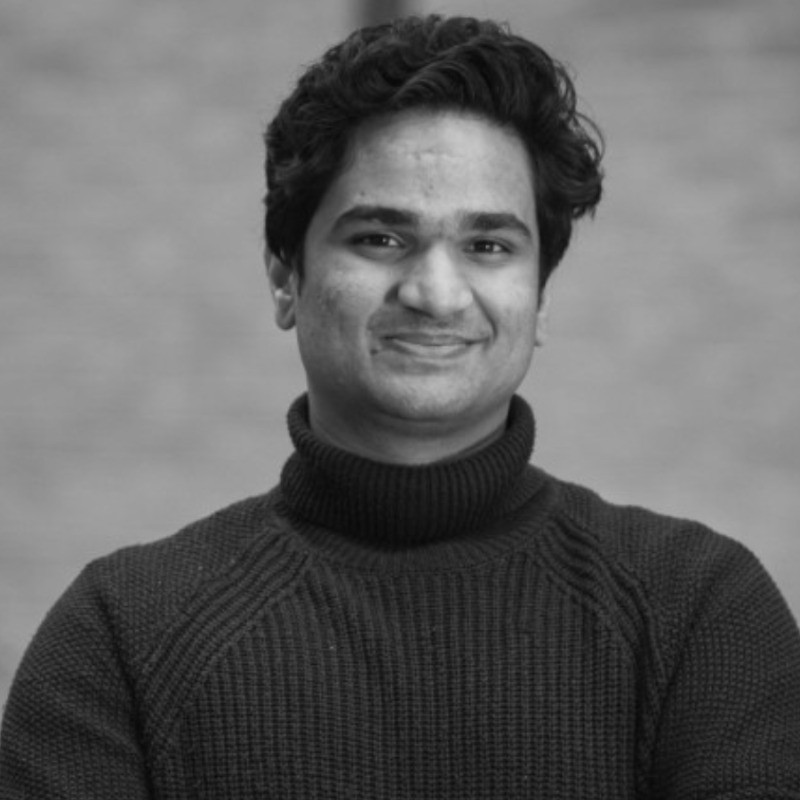
\includegraphics[width=2.3cm,height=2.3cm,keepaspectratio]{photo.jpg}
\end{minipage}

\section{Career Summary}
\begin{itemize}
\item Automation Engineer with dual degrees in Mechanical Engineering and Management Engineering (Politecnico di Milano), specializing in industrial automation systems and PLC development.
\item Solid foundation in Siemens TIA Portal programming (S7-1200 / S7-1500), Siemens HMI design, and field commissioning of automated industrial lines.
\item Practical experience configuring industrial networks (PROFINET, PROFIBUS, Modbus TCP/RTU, OPC UA), inverter drives, servo-actuators, and field instrumentation.
\item Skilled in reading electrical schematics, diagnosing software/hardware anomalies during collaudo, and drafting comprehensive technical operating procedures.
\end{itemize}

\section{Technical Skills}
\begin{itemize}
\item \textbf{PLC \& HMI Programming} -- Siemens TIA Portal (S7-1200, S7-1500), WinCC HMI, Ladder Logic (LAD), Structured Text (SCL), Function Block Diagram (FBD)
\item \textbf{Industrial Field Networks} -- PROFINET, PROFIBUS, Modbus TCP/RTU, OPC UA, Industrial Ethernet, Fieldbus Gateways
\item \textbf{Drives \& Motion Control} -- Frequency Inverters, Servo-drives, Stepper Motors, Sensors, Electrical Schematics \& Wiring Diagrams
\item \textbf{Testing \& Commissioning} -- Plant Commissioning (Collaudo), FAT/SAT Protocols, Software Fault Isolation, Hardware Diagnostics
\item \textbf{Languages \& Tools} -- Python, C++, Bash, SQL, Git, Linux, Technical Documentation
\end{itemize}

\section{Visa \& Language}
\begin{itemize}
\item \textbf{Language} -- Italian (Conversational / Intermediate), English (Fluent / Professional), Hindi (Native)
\item \textbf{Work Authorization} -- European Long Term Residence Permit (No Visa Sponsorship required). Italian Partita IVA active. Driving License (Patente B). Available for on-site travel and commissioning.
\end{itemize}

\section{Professional Experience}
\role{\href{https://flowspace.co}{FlowSpace.co}}{Automation \& Systems Lead}{London, UK / Remote}{Mar 2024 -- Ongoing}
\begin{itemize}
\item \textbf{Systems Engineering \& Diagnostic Tooling:}
\begin{itemize}[label=--]
\item Designed automated monitoring and testing pipelines for industrial systems and edge devices, verifying data throughput and cycle reliability.
\item Built automated health diagnostics capturing communication timeout events and sensor telemetry anomalies in real time.
\item Formulated technical operating procedures and system documentation for deployment and commissioning teams.
\end{itemize}
\item \textbf{Hardware-Software Integration:}
\begin{itemize}[label=--]
\item Interfaced multi-protocol field devices with central control logic via Modbus and industrial network bridges.
\item Maintained 99.9\% uptime across critical operational workflows through proactive troubleshooting and routine firmware verification.
\end{itemize}
\item \textit{Tools: Python, Linux, Bash, Industrial Networks, Modbus, Docker, Git}
\end{itemize}

\role{Urlink}{Systems Automation Engineer}{Milan, Italy}{Jul 2023 -- Feb 2024}
\begin{itemize}
\item Assisted in the commissioning and acceptance testing (collaudo) of automated industrial machinery at manufacturing customer facilities.
\item Programmed and verified PLC I/O logic, safety interlocks, and sensor feedback loops in compliance with electrical schematics.
\item Configured industrial networking switches, drive parameters, and operator panels for reliable field execution.
\end{itemize}

\role{UltraStrategy}{Automation Developer}{Remote, Germany}{Sep 2022 -- Jun 2023}
\begin{itemize}
\item Developed automated scripts monitoring industrial equipment status, cycle times, and operational performance metrics.
\item Created automated diagnostic routines summarizing machine health for quality assurance audits.
\end{itemize}

\section{Education}
\role{Politecnico di Milano}{M.Sc. in Management Engineering (Digital Business \& ICT)}{Milan, Italy}{2020 -- 2023}
\role{Thapar Institute of Engineering and Technology}{B.E. in Mechanical Engineering}{Punjab, India}{2014 -- 2018}

\end{document}
